\documentclass[a0,portrait]{sciposter}
%\usepackage[brazil]{babel}
\usepackage[utf8]{inputenc}
\usepackage[centertags]{amsmath}
\usepackage{amsfonts,multirow,multicol}
\usepackage{graphicx,colortbl}
\usepackage{geometry}
\geometry{paperwidth=83.96cm,paperheight=118.82cm,centering,textwidth=75cm,textheight=115cm,left=3cm,top=3cm}
%\geometry{paperwidth=90cm,paperheight=100cm,centering,textwidth=77cm,textheight=89cm,left=3cm,top=3cm}
%\pagestyle{plain}
\frenchspacing

\usepackage{pgfplots}
\usetikzlibrary{positioning, backgrounds}

\usepackage{adjustbox}


\usepackage{pgfplotstable}
\usepgfplotslibrary{colorbrewer}
\pgfplotsset{compat=1.15}
\usepgfplotslibrary{statistics}
\pgfplotstableread{%
    Author min avg max mediana deviation
    ClercA 100.1900 131.5194 180.2100 130.2000 16.0537
    ClercB 100.1900 131.9290 190.2000 130.2000 15.6576
    ClercC 100.1900 145.2007 210.2000 140.2100 17.3981
    ClercD 100.1900 113.8061 150.2100 110.2000 10.8342
    ClercE 100.1900 131.7290 180.2000 130.2000 15.7357
    EberhartA 100.1900 129.8890 170.2100 130.2000 15.8132
    EberhartB 100.1900 127.4685 170.2000 130.1900 14.4167
    EberhartC 100.2000 142.6508 190.2100 140.2000 16.6241
    EberhartD 100.1800 113.9665 150.2100 110.2000 11.2164
    EberhartE 100.1900 129.6588 190.2100 130.2000 15.0647
    XinA 100.1900 126.8997 170.2000 130.2000 14.3637
    XinB 100.1900 124.3386 170.2000 130.1900 13.5221
    XinC 100.1900 137.3308 190.2000 130.2100 16.0478
    XinD 100.1800 113.8771 160.2000 110.2000 11.1794
    XinE 100.1800 126.7993 180.2100 130.1900 14.4938
}\datatable


%%Transformando tudo em branco
\renewcommand{\thesection}{\textcolor{white}{\arabic{section}}}
\renewcommand{\thesubsection}{\textcolor{white}{\arabic{section}.\arabic{subsection}}}



%%rodape feito com TikZ
\newcommand{\rodape}[2]{
    \begin{tikzpicture}[remember picture,overlay]
    \node at (current page.south west){
        \begin{tikzpicture}[remember picture,overlay,inner sep=0,outer sep=0]
        \draw[fill=#2] (0,0) rectangle (.93\paperwidth,3);
        \node[above right] at (4cm,0.2) {
            \includegraphics[height=2.5cm]{#1} %%terceiro logo
        };
        \end{tikzpicture}
    };
    \node[yshift=2cm,yellow] at (current page.south){\color{white}{This study was financed in part by Instituto Federal do Paraná and the Coordenação de Aperfeiçoamento de Pessoal de Nível Superior -- Brasil (CAPES) -- Finance Code 001.}};
\end{tikzpicture}
}


%%Definindo cores
\definecolor{BoxCol}{RGB}{71,109,239} %azul



\newcommand{\tituloA}[1]{\emph{\textbf{\color{white}{#1}}}}
\newcommand{\tituloB}[1]{\emph{\textbf{\color{blue}{#1}}}}
\renewenvironment{abstract}
{\section*{\color{white}{\abstractname}}\it}
{}




\begin{document}

\setlength{\abovedisplayskip}{2pt}
\setlength{\belowdisplayskip}{2pt}

%%titulo
\colorbox{BoxCol}{
  \begin{minipage}{\textwidth}
    \color{white}{
     \begin{center}
        \huge{\textbf{\vspace{1cm} \\
          Analysis of the PSO parameters for a robots positioning system in SSL %insira o titulo aqui
        \vspace{1cm} \\}}
      \end{center}
    }
  \end{minipage}
}

\rodape{qrcode}{BoxCol} %azul

\title{}
\author{Marcos Aurelio Pchek Laureano $^{1,2}$, Flavio Tonidandel $^2$} %%<-- seu nome
    \institute{$^1$ Federal Institute of Parana, Curitiba -- PR, Brazil
    \\
    $^2$ University Center of FEI, São Bernardo do Campo -- SP, Brazil}

    \email{$^1$ marcos.laureano@ifpr.edu.br, $^2$ flaviot@fei.edu.br}
\leftlogo[1]{logo} %logotipo da universidade
%\rightlogo[1]{qrcode} %logotipo da universidade


\maketitle %gera titulo

\colorbox{BoxCol}{
  \begin{minipage}{\textwidth}
    \begin{center}
      \vspace{0.5cm}
      %digite o nome do congresso aqui
      \color{white}{\Large{The 23rd Annual RoboCup International Symposium 2019 \qquad --- \qquad \textbf{RoboCup 2019}}}
      \vspace{0.5cm} 
    \end{center}
  \end{minipage}
}

%Texto em 3 colunas
\begin{multicols}{3}

%Paragrafo.
\setlength{\parindent}{3em}

\begin{abstract}
    The changes in the Small Size League rules have brought greater possibilities of playing. With the increased complexity of soccer matches, the positioning of the robots has become important as a defense and attack mechanism. The learning of opposing team game playing has been shown to be effective, but an SSL soccer match indicates the need for solutions that analyze the strategy of the opposing team during the game and make any necessary adaptations. This paper proposes the use of the Particle Swarm Optimization (PSO) algorithm as an option to determine the positioning during the match. A prototype has been developed to validate the configuration parameters. Experiments in a simulator, analysis of game logs and results in a real matches have demonstrated the feasibility of applying the PSO algorithm to find the robots positions.
\end{abstract}

\section*{\tituloA{Particle Swarm Optimization}}
    \PARstart{P}article swarm optimization (PSO) is a computational method that optimizes a problem by iteratively trying to improve a candidate solution with regard to a given measure of quality. It solves a problem by having a population of candidate solutions, here called particles, and moving these particles around in the search space according to the mathematical formula over the particles position and velocity.


\subsection*{\tituloB{PSO pbest and gbest equation}}
    \[
        \begin{aligned}
    pbest(i,t) = min [ f(P_i(k))], i \in {1,...,N_p}, k=1,...,t 
    \\
    gbest(t) = min [ f(P_i(k))], i = 1,...,N_p,  k=1,...,t
    \end{aligned}
    \]

\subsection*{\tituloB{PSO Velocity equation}}
    \[
    \begin{aligned}
    V_i(t+1) =&\underbrace{\underbrace{\omega V_i(t)}_{ \textrm{inertia} }}_{\textrm{diversification}} +\\ 
    &\underbrace{\underbrace{c_1 r_1 ( pbest(i,t) - P_i(t) )}_{\textrm{cognitive}} + 
        \underbrace{c_2 r_2( gbest(t)-P_i(t) )}_{\textrm{social}}}_{\textrm{intensification}}
    \end{aligned}
    \]


\subsection*{\tituloB{PSO Position equation}}
    \[
    \begin{aligned}
    P_i(t+1)=P_i(t) +V_i(t+1)
    \end{aligned}
    \]

\section*{\tituloA{Proposal}}
    \PARstart{T}he first objective is to test, verify, and determine the configuration parameters (inertia, confidence, number of iterations and population size) of the PSO algorithm in order to optimize robot positioning in the field. The second is to demonstrate the effective positioning of robots based on the defense fitness function developed for this study.


    To meet the defense requirements similar to those in human soccer, a fitness evaluation function is used in simulations applied to the defense position. 

    It evaluates four desirable situations for a defense formation:
    \begin{itemize}
        \item A minimum distance among the robots in order to make opponent's movements more difficult and decrease the opponent's chances to receive the ball, make passes or kick to goal; 
        \item The view of the opponent's robots in relation to a certain point of interest is blocked;
        \item The view of the goal of all the opponent's robots is blocked by least one robot of team, especially opponent robot with ball possession;  
        \item Respect for the SSL rules on collisions between robots and invasion of the goal area. 
    \end{itemize}



\section*{\tituloA{General Equation}}
    \PARstart{F}ield size is considered in centimeters and the \emph{Goal} term can be any point of interest in the search space.

    \[
    \begin{aligned}
    \operatorname{fitness}(A, p(i,t),goal) =  
    & \operatorname{f_{MinDistance}}(A, p(i,t)) + \\
    & \operatorname{f_{CheckStraight}} (A, p(i,t), goal) + \\
    & \operatorname{f_{ProtectGoal}}(A, p(i,t)) + \\
    & \operatorname{f_{Colission}}(A, p(i,t)) + \\
    & \operatorname{f_{InvasionGoalArea}}(p(i,t))
    \end{aligned}
    \
    \]

\subsection*{\tituloB{Minimum distance}}

    \[
    \begin{aligned}
        \operatorname{f_{MinDistance}}(A, P) = \{\\
        & \operatorname{distance}(p,a) = \sqrt{ (p_x-a_x)^2  + (p_y - a_y)^2}\\
        & d = \operatorname{distance}(p,a) \\
        & I_{c_{d}}(p,a) = \begin{cases}
        (1-\frac{40}{d}), & \text{ if } (1-\frac{40}{d}) >0  \\ 
        \mathop{\text{\textsc{PMID}}}, & \text{otherwise} 
        \end{cases}
        \\
        & \sum_{a \in A} \sum_{p \in P} \ I_{c_{d}}(p,a) \\ \}
    \end{aligned}
    \]


\subsection*{\tituloB{Blocking the view of points of interest}}

    \[
    \begin{aligned}
        \operatorname{f_{CheckStraight}} (A, P, goal)= \{ \\
        &\operatorname{straight}(a,p,g) = \{ ((g_y - p_y) \times a_x + \\ 
        & (p_x - g_x) \times a_y + (g_x \times p_y - p_x \times g_y)) \}
        \\
        & s = \begin{cases}
        0, & \text{ if } a \ \text{has the ball} \\ 
        \mathop{\text{\textsc{PLOW}}}, & \text{ otherwise }
        \end{cases}
        \\
        & I_{c_{s}}(p,a,goal) = \operatorname{straight}(a,p,goal) + s
        \\
        & \sum_{a \in A} \sum_{p \in P} \ I_{c_{s}}(p,a,goal) \\
        \}
    \end{aligned}
    \]

\subsection*{\tituloB{Blocking the view of the goal}}

    \[
    \begin{aligned}
        \operatorname{f_{ProtectGoal}}(A,P) = \mathop{\text{\textsc{PMID}}} \times ( \sum_{p \in P}  \ \forall \ p \notin A_{ball} )
    \end{aligned}
    \]



\subsection*{\tituloB{Respect SSL rules}}
    \[
    \begin{aligned}
        \operatorname{f_{Colission}}(A, P) = & \mathop{\text{\textsc{PHIGH}}} \times ((\sum_{a \in A} \sum_{p \in P} \operatorname{pos}(a) = \operatorname{pos}(p) + \\
        & (\sum_{p \in P} \sum_{q \in P} \operatorname{pos}(p) = \operatorname{pos}(q) \ \land \ p_{id} \neq q_{id}))
    \end{aligned}
    \]

    \[    
    \begin{aligned}
        \operatorname{f_{InvasionGoalArea}}(P) = \mathop{\text{\textsc{PHIGH}}} \times (\sum_{p \in P} \forall \ p \in \textrm{Goal area})
    \end{aligned}
    \]
    
\section*{\tituloA{Discovery best PSO parameters}}
    \PARstart{I}nertia weight ($\omega$) plays a key role in providing balance in the local and global exploitation process. $\omega = 0.7298$, $\omega = 0.5 + \frac{rand(0,1)}{2}$ and  $\omega = (\omega_{start} - \omega_{end}) \times \frac{it_{Max} - it}{it_{Max}} + \omega_{end}$ 
\\

    Fifteen simulation scenarios to find parameters $\omega$, $c_1$ and $c_2$. 15 seconds of movement to simulate a real game situation; The population size (from 50 to 200); Number of iterations (from 50 to 500); Global and local best neighborhood topologies were used. 
\\

\subsection*{\tituloB{Results}}

    \begin{figure}[h!]
    \begin{adjustbox}{width=1\linewidth,center}
    \begin{tikzpicture}
        \pgfplotstablegetrowsof{\datatable}
        \pgfmathtruncatemacro{\rownumber}{\pgfplotsretval-1}
        \begin{axis}[boxplot/draw direction=y,
        xticklabels={ClercA,ClercB,ClercC,ClercD,ClercE,EberhartA, EberhartB, EberhartC, EberhartD, EberhartE,XinA, XinB, XinC, XinD, XinE},
        xtick={1,...,\the\numexpr\rownumber+1},
        x tick label style={scale=0.3,font=\bfseries, rotate=90,,align=center},
        ylabel={fitness}, ylabel style={scale=0.5,font=\bfseries,align=center},
        y tick label style={scale=0.5,font=\bfseries,align=center},,
        cycle list/PuBu-6 , 
        colormap={myColor}{
            indices of colormap=(2,...,\pgfplotscolormaplastindexof{PuBu-6} of PuBu-6)},
        cycle list/.define={myColor}{[of colormap=myColor]},
        cycle list name=myColor,
        ]
            \pgfplotsinvokeforeach{0,...,\rownumber}{
                
                \pgfplotstablegetelem{#1}{min}\of\datatable
                \edef\mymin{\pgfplotsretval}
                
                \pgfplotstablegetelem{#1}{avg}\of\datatable
                \edef\myavg{\pgfplotsretval}
                
                \pgfplotstablegetelem{#1}{max}\of\datatable
                \edef\mymax{\pgfplotsretval}
                
                \pgfplotstablegetelem{#1}{mediana}\of\datatable
                \edef\mymediana{\pgfplotsretval}
                
                \pgfplotstablegetelem{#1}{deviation}\of\datatable
                \edef\mydeviation{\pgfplotsretval}
                
                \typeout{\mymin,\mymax,\myavg,\mymediana,\mydeviation}
                \pgfmathsetmacro{\mylowerq}{\mymediana-\mydeviation}
                \pgfmathsetmacro{\myupperq}{\mymediana+\mydeviation}
                \edef\temp{\noexpand\addplot+[,
                    boxplot prepared={
                        lower whisker=\mymin,
                        upper whisker=\mymax,
                        lower quartile=\mylowerq,
                        upper quartile=\myupperq,
                        median=\myavg,
                        every box/.style={solid,fill,opacity=0.7,draw=black},
                        every whisker/.style={solid,draw=black },
                        every median/.style={solid,draw=black},
                    }, 
                    ]coordinates {};}
                \temp
            }
        \end{axis}
    \end{tikzpicture}    
    \end{adjustbox}
    {\small Scenario settings: a) $c_1 = 1$ and $c_2 = 2$; b) $c_1 = 2$ and $c_2 = 1$; c) $c_l = c_2 = 1$; d) $c_1 = c_2 = 2$ and e) $c_1 = c_2 = 1.496$.}
    \end{figure}


    All scenarios with $c_1 = c_2 = 2$ have the best results, followed by the scenario with $c_1 = c_2 = 1.496$.
\\ %quebra linha

\section*{\tituloA{Experiments}}
    \PARstart{T}hree types of experiment were performed using PSO equations with parameters $\omega=0.7298, c_1=c_2=2$ to calculate the velocity and position of each robot that make up the particle, a grSim simulator, log analysis of RoboCup 2018 and the \emph{Latin American Robotics Symposium} 2018 (LARS 2018) in five real matches.
\\

\subsection*{\tituloB{Results -- Simulator}}
    In the grSim simulator, the ball and the opponent's robots were positioned differently for visual verification of the behavior of the team robots. These validations allowed us to identify and adjust some parameters of the fitness function.
\\

\subsection*{\tituloB{Results -- RoboCup 2018 playoffs}}
    Five matches were selected from the RoboCup 2018 playoffs. Each scenario was evaluated 1,000 times with the parameters of the algorithm found in the previous experiments.


    \begin{adjustbox}{width=1\linewidth, center}
        \begin{tikzpicture}[framed]
        \centering
        \begin{axis}[
        ybar, axis on top,
        title={Interception of ball during the pass or goal kick},
        height=8cm, width=.25\textwidth,
        bar width=1cm,
        ymajorgrids, tick align=inside,
        major grid style={draw=white},
        enlarge y limits={value=.1,upper},
        ymin=0, ymax=100,
        axis x line*=bottom,
        axis y line*=right,
        y axis line style={opacity=0},
        tickwidth=0pt,
        enlarge x limits=true, %scale=.5,
        legend style={
            at={(0.5,-0.2)},
            anchor=north,
            legend columns=-1,
            /tikz/every even column/.append style={column sep=0.5cm}
        },
        ylabel={Percentage (\%)},
        symbolic x coords={
            Match 1,Match 2,Match 3, Match 4, Match 5},
        xtick=data,
        nodes near coords={
            \pgfmathprintnumber[precision=0]{\pgfplotspointmeta}
        }
        ]
            \addplot [draw=none, fill=blue!30] coordinates {
                (Match 1,89.05)
                (Match 2, 87.76) 
                (Match 3,88.91)
                (Match 4,92.93) 
                (Match 5,91.43) };
            
            
            \addplot [draw=none, fill=green!30] coordinates {
                (Match 1,75.4064)
                (Match 2, 79.7961) 
                (Match 3,74.4597)
                (Match 4,76.6786) 
                (Match 5,77.5600) };
            
            
            \legend{Gol,Pass}
        \end{axis}
        \end{tikzpicture}
    \end{adjustbox}
\\

\subsection*{\tituloB{Results -- LARS 2018 matches}}
    These experiments allowed us to verify the positioning limitations caused by the time spent in processing and sending commands to the robots. In games with dead-ball situations, the positioning found by the system was always a difficult one for passes or kicks to goal.

\section*{\tituloA{Conclusions}}

    \begin{figure}[h!]
        \centering
        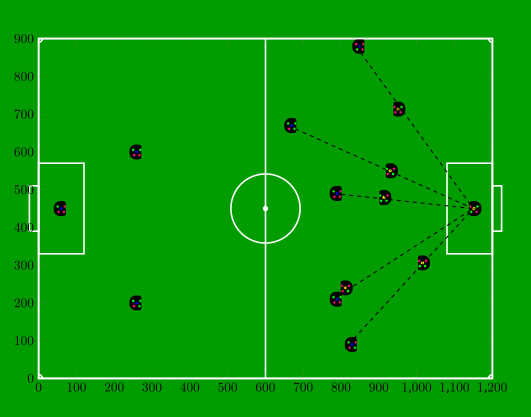
\includegraphics[width=1\linewidth]{resultadoclerc2002.png}
        {\small Example of positioning}
    \end{figure}

    \PARstart{T}he experiments indicate that the best global neighborhood topology, the number of iterations (300), acceleration coefficients ($c_1=c_2=2$), and the size of the population (100) meet the project requirements in terms of computational costs to be run during a real soccer match. For inertia, all the evaluated strategies were effective, and we adopted the value $\omega=0.7298$.

    The analysis of RoboCup playoff logs has demonstrated the effectiveness of the proposal for this paper. Experiments conducted during LARS 2018 have shown that it can be used to find field positioning during an real SSL soccer game, especially in games with dead-ball situations (e.g. indirect kicks). However, for a dynamic game, the movements of the opponent's must be considered in order to calculate the future positioning, which is the main challenge to be improved on future studies.


\end{multicols}

\end{document} 